\documentclass[english,12pt,a4paper,pdftex]{article}
\usepackage[english]{babel}
\selectlanguage{english}
\usepackage[utf8]{inputenc}
\usepackage[elec,utf8]{aaltothesis}
\usepackage{graphicx}
\usepackage{url}
\usepackage[pdfpagemode=FullScreen,colorlinks=true,urlcolor=red,%
linkcolor=blue,citecolor=black,pdfstartview=FitH]{hyperref}
\usepackage{amsfonts,amssymb,amsbsy}

%% Vaakasuunnan mitat, äLä KOSKE!
\setlength{\hoffset}{-1in}
\setlength{\oddsidemargin}{35mm}
\setlength{\evensidemargin}{25mm}
\setlength{\textwidth}{15cm}
%% Pystysuunnan mitat, äLä KOSKE!
\setlength{\voffset}{-1in}
\setlength{\headsep}{7mm}
\setlength{\headheight}{1em}
\setlength{\topmargin}{25mm-\headheight-\headsep}
\setlength{\textheight}{23cm}

\newcommand{\publishedDate}{00.00.2014}

\begin{document}

\department{Department of Automation and Systems Technology}%
{Automaatio- ja systeemitekniikan laitos}
\professorship{Media Technology}{Viestintätekniikka}
\code{AS-75}

\univdegree{MSc}
\author{Marko Raatikka}

\thesistitle{LuminoTrace: a mobile approach to cost-effective product authentication}{LuminoTrace: kustannustehokas aitoudentunnistus mobiililaitteella}

\place{Espoo}

\date{\publishedDate{}}

\supervisor{Prof.\ Petri Vuorimaa}{Prof.\ Petri Vuorimaa}
\instructor{D.Sc.\ (Tech.) Jari Kleimola}{TkT Jari Kleimola}
\instructor{Prof.\ (Tech.) Jouni Paltakari}{Prof.\ Jouni Paltakari}

% \uselogo{aaltoRed|aaltoBlue|aaltoYellow|aaltoGray|aaltoGrayScale}{?|!|''}
\uselogo{aaltoBlue}{''}

\makecoverpage

\keywords{photoluminescence, smartphone, web application, authenticity}
\begin{abstractpage}[english]
 % Your abstract in English. Try to keep the abstract short, approximately
 % 100 words should be enough. Abstract explains your research topic,
 % the methods you have used, and the results you obtained.


\end{abstractpage}

\newpage

%% Finnish abstract
\keywords{fotoluminesenssi, älypuhelin, web-sovellus, aitoudentunnistus}
\begin{abstractpage}[finnish]
%% ...
\end{abstractpage}

\mysection{Acknowledgments}

\vspace{1cm}
\noindent Espoo, \publishedDate{}\\

\vspace{0.15cm}
\noindent Marko Raatikka

\newpage

\thesistableofcontents

%% Symbols and abbreviations
\mysection{Abbreviations and Acronyms}

\begin{tabular}{ll}
AC         & vaihtovirta \\
APLAC      & an object-oriented analog circuit simulator and design tool \\
           & (originally Analysis Program for Linear Active Circuits) \\
BCS        & Bardeen-Cooper-Schrieffer \\ %% tavuviiva - nimien välissä
DC         & tasavirta \\
TEM        & transverse eletromagnetic
\end{tabular}

\cleardoublepage
\storeinipagenumber
\pagenumbering{arabic}
\setcounter{page}{1}


\section{Introduction}
% Johdanto selvittää samat asiat kuin tiivistelmä, mutta laveammin. Johdannossa kerrotaan yleensä seuraavat asiat

% \begin{itemize}
% \item[--]Tutkimuksen taustaa ja tutkimusaiheen yleisluonteinen esittely
% \item[--]Tutkimuksen tavoitteet
% \item[--]Pääkysymys ja osaongelmat
% \item[--]Tutkimuksen rajaus ja keskeiset käsitteet.
% \end{itemize}

\subsection{Research questions}
\subsection{Outline}

\thispagestyle{empty}
The focus of this thesis is the design and implementation of a scalable hybrid mobile application. The application will be developed as a part of the LuminoTrace project at Aalto CHEM for the purposes material verification. The functionality of the application can be briefly described as follows:

\begin{enumerate}
\item A user takes an image of a material with his/her mobile device
\item An algorithm analyzes the image and returns a unique digital fingerprint
\item The fingerprint is compared against a database of fingerprints
\item The user is notified whether or not a match was found.
\end{enumerate}

The verification is done by analyzing the spectrum of a special chemical compound embedded in the material. Both the underlying algorithm and the compound have already been developed as a part of the LuminoTrace project.

The implementation of the application can be divided into the following tasks:

\begin{itemize}
\item[--]Access and control built-in camera of the mobile device
\item[--]Port the code of the spectrum analysis algorithm to JavaScript
\item[--]Implement the UI
\item[--]Implement the back end infrastructure (cloud)
\end{itemize}

\begin{figure}[hbs]
\centering 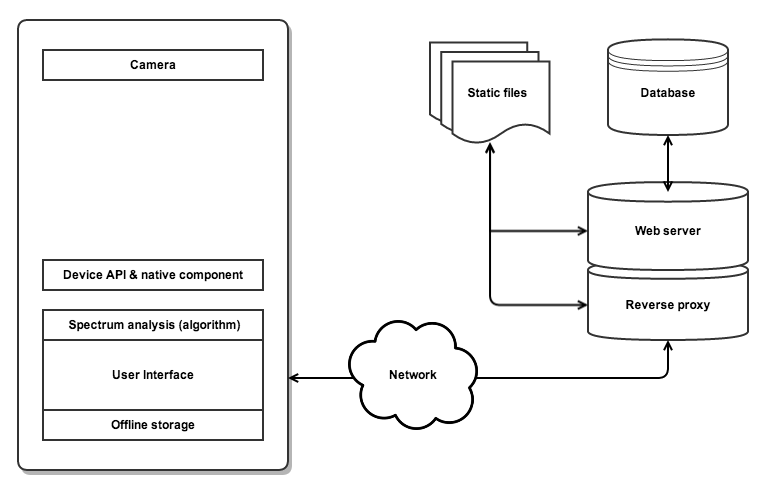
\includegraphics[width=13.25cm]{assets/diagram_0404}
\caption{A high-level overview of the structure of the application \label{diagram}}
\end{figure}

The functionality outlined above can be largely achieved by utilizing existing Web technologies and the W3C Device APIs. However, a more granular control over the camera (e.g. burst-mode, flash settings) will require a native component to be implemented for each target platform. The preliminary target platform will be Windows Phone (WP). To improve scalability the fingerprint will be computed on the client-side. This will require for the existing algorithm to be ported into JavaScript. Scalability can be further improved by offloading parts of the (fingerprint) database from the server to the user's device. Moreover, usability is improved as the application can function offline without the overhead of network latency. Hosting fingerprint data on the user's device might however have security implications: can the data be safely/efficiently encrypted on the user's device?

The underlying server back end will consist of a web server and a database to hold the fingerprint data. Optionally, a reverse proxy can be set up in front of the web server to allow static assets to be served to the client without hitting the web server. However, since the application will most likely not include many static assets (images, JS, CSS...) the benefit of this is somewhat minimal. The back end will be implemented using Node.js due to its convenience (author's previous experience and the possibility to re-use the ported spectrum algorithm both in the front and back end). The database will be implemented with MongoDB as it couples well with Node.js and has cross-platform support and an active community.

A high-level overview of the main components and interfaces of the application described above is given in Figure \ref{diagram}.

Hybrid apps are essentially small websites running in a browser shell in an app that have access to the native platform layer. Hybrid apps have many benefits over pure native apps, specifically in terms of platform support, speed of development, and access to 3rd party code.

%% In a thesis, every section starts a new page, hence \clearpage
\clearpage

\section{Background}

Tässä osassa selvitetään, mitä tutkimuksen kohteena olevasta
aiheesta tiedetään entuudestaan. Selvityksen tulee kattaa
tasapainoisesti koko tutkimuskenttä.

\subsection{Existing solutions}

\subsection{Mobile Platforms, Tools and Frameworks}

\subsection{Hybrid Applications}

\subsection{Photoluminescence}

\subsection{RGB and HSV color spaces}

\subsection{Pixel Formats}

\subsection{Mobile Camera Technology}

\begin{table}[htb]
%% Taulukon teksti
\caption{Taulukoissa ja kuvissa kirjaintyypin voi valita
tarkoituksenmukaisesti, mutta kuva- ja taulukkoteksteissä tulee
käyttää samaa kirjaintyyppiä kuin varsinaisessa tekstissä.
Huomaa taulukon numeroinnin sijoittuminen taulukon yläpuolelle. \label{taulukko1}}
\begin{center}
\fbox{
	\begin{tabular}{c|l|r}
	\textbf{A} & 1 & $e^{j \omega t}$ \\ \hline
	\textsf{B} & 2 & ${\mathfrak R}(c)$ \\ \hline
	\texttt{C} & 3 & $ a \in \mathbb{A}$
	\end{tabular}
}
\end{center}
\end{table}

%% Kaavojen jälkeen ei yleensä laiteta sisennystä.
\begin{equation}
D(xy) = (Dx)y + x(Dy),  \hspace{3em} x,y \in \mathbb{A}.
\end{equation}

\begin{figure}[htb]
\centering 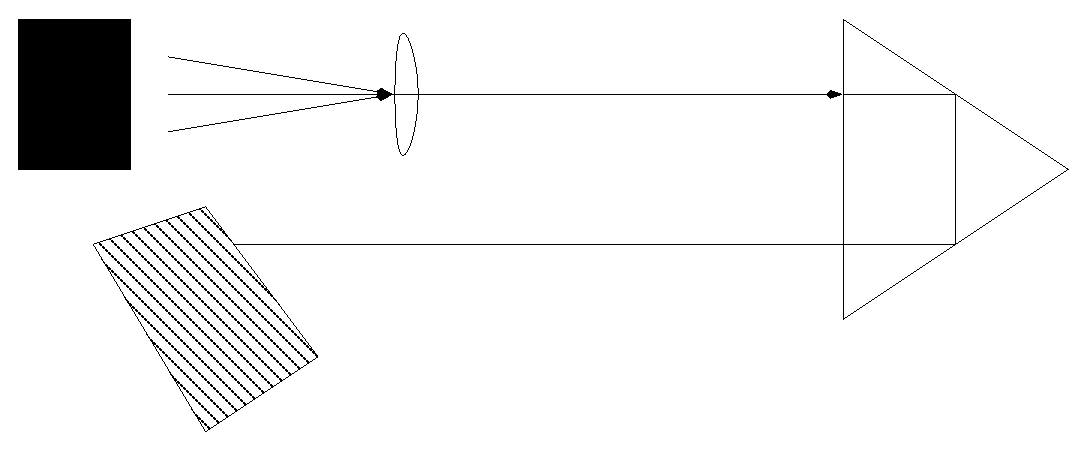
\includegraphics[height=5cm]{assets/kuva1}
\caption{Tämä on esimerkki numeroidusta kuvatekstistä. \label{kuva1}}
\end{figure}

%% Esimerkki korostamisesta. Lihavoinnin sijasta on tyylikkäämpää
%% ja luettavampaa käyttää kursiivia.

\clearpage

\section{Design and Implementation}

Tässä osassa kuvataan käytetty tutkimusaineisto ja
tutkimuksen metodologiset valinnat, sekä
kerrotaan tutkimuksen toteutustapa ja käytetyt menetelmät.

\subsection{Requirements}

R1, R2, R3... (mitattavia suureita)

% \subsection{Application architecture}

\subsection{User Interface}

\subsection{Camera Module and Setup}

\subsection{Server Backend and Storage}

\subsection{Authenticity Verification Process}

\subsubsection{Peak Finding}

\subsubsection{Similarity Matching}

\clearpage

\section{Evaluation and discussion}
\subsection{Algorithmic Robustness}
\subsection{Performance Analysis}
\subsection{Problem Space and Challenges}

% Tässä osassa esitetään tulokset ja vastataan tutkielman alussa
% esitettyihin tutkimuskysymyksiin. Tieteellisen kirjoitelman
% arvo mitataan tässä osassa esitettyjen tulosten perusteella.
% Tutkimustuloksien merkitystä on aina syytä arvioida ja tarkastella
% kriittisesti. Tässä osassa on syytä myäs arvioida tutkimustulosten luotettavuutta.

\clearpage

\section{Conclusions}

No offical API, no fine grained control over the camera (ISO, shutter speed)
JavaCPP, Xamarin
Developer convenience
Future work (isot kokonaisuudet!)

\clearpage

\phantomsection
\addcontentsline{toc}{section}{References}
\begin{thebibliography}{99}

% Kirja
%% Alla pilkun jälkeen on pakotettu oikea väli \<välilyänti>-merkeillä.
\bibitem{Kauranen} Kauranen,\ I., Mustakallio,\ M. ja Palmgren,\ V.
  \textit{Tutkimusraportin kirjoittamisen opas opinnäytetyän
    tekijäille.}  Espoo, Teknillinen korkeakoulu, 2006.

\bibitem{Koblitz} Koblitz,\ N. \textit{A Course in Number Theory and
    Cryptography. Graduate Texts in Mathematics 114.}  2.\ painos. New
  York, Springer, 1994.

\bibitem{Itkonen} Itkonen,\ M. \textit{Typografian käsikirja.} 3.\
  painos.  Helsinki, RPS-yhtiät, 2007.

% Artikkeli
%% Kun on useampi nimikirjain, jokaisen nimikirjaimen väliin
%% kuuluu välilyänti. Oikea välin määrä on saatu \<välilyännillä>
\bibitem{bcs} Bardeen,\ J., Cooper,\ L.\ N. ja Schrieffer,\ J.\ R.
  Theory of Superconductivity. \textit{Physical Review,} 1957, vol.\
  108, nro~5, s.\ 1175--1204.

\bibitem{Deschamps} Deschamps,\ G.\ A. Electromagnetics and
  Differential Forms. \textit{Proceedings of the IEEE,} 1981, vol.\
  69, nro~6, s.\ 676--696.

% Kokoomateos
%% Alla esimerkki englanninkielisen tavuttamisen pakottamisesta.
%% Oletusarvoisesti käytetään suomalaista tavutusta, mutta viitteissä
%% esiintyy usein muunkielisiä lauseita, jotka tulevat siten tavutetuksi
%% suomen kielen sääntäjen mukaan. Tämän voi korjata \foreignlanguage-
%% komennolla, jonka ensimmäinen parametri on vieraan kielen nimi ja toinen
%% on vieraalla kielellä tavutettava teksti.
\bibitem{Sihvola} Sihvola,\ A.\ et al.
  \foreignlanguage{english}{Interpretation of measurements of helix
and bihelix superchiral structures.}  Teoksessa: Jacob,\ A.\ F. ja
  Reinert,\ J. (toim.) \textit{Bianisotropics '98 7th International
    Conference on Complex Media.}  Braunschweig, 3.--6.6.1998.
  Braunscweig, Technische Universität Braunschweig, 1998, s.\
  317--320.

% Opinnäytetyö
%% Alla on suomalainen yhdistelmäsukunimi. Sen nimien välissä
%% käytetään yhdysmerkkiä l. tavuviivaa, kirjoitetaan -.
\bibitem{Lindblom} Lindblom-Ylänne,\ S. ja Wager,\ M.  Tieteellisten
  opinnäytetäiden ohjaaminen. Teoksessa: Lindblom-Ylänne,\ S. ja
  Nevgi,\ A. (toim.) \textit{Yliopisto- ja korkeakouluopettajan
    käsikirja.}  Helsinki, WSOY, 2004, s.\ 314--325.

\bibitem{Miinusmaa} Miinusmaa,\ H. Neliskulmaisen reiän poraamisesta
  kolmikulmaisella poralla. Diplomityä, Teknillinen korkeakoulu,
  konetekniikan osasto, Espoo, 1977.

% Standardista
\bibitem{sfs} SFS 5342. Kirjallisuusviitteiden laatiminen. 2.\ painos.
  Helsinki, Suomen standardisoimisliitto, 2004. 20~s.

% Haastattelusta
\bibitem{haastattelu} Palmgren,\ V. Suunnittelija. Teknillinen
  korkeakoulu, kirjasto. Otaniementie 9, 02150 Espoo. Haastattelu
  15.1.2007.

% Vain verkosta saatavissa olevasta artikkelista
\bibitem{kone} Pohjois-Koivisto,\ T. Voiko kone tulevaisuudessa arvata
  tahtosi?  \textit{Apropos,} verkkolehti, helmikuu, nro~1, 2005.
  Viitattu 19.1.2007.  Saatavissa:
  \url{http://www.apropos.fi/1-2005/prima.php.}

\bibitem{Ribeiro} Ribeiro,\ C.\ B., Ollila,\ E. ja Koivunen,\ V.
  \foreignlanguage{english}{Stochastic Maximum-Likelihood Method for
    MIMO Propagation Parameter Estimation.} \textit{IEEE Transactions
    on Signal Processing,} verkkolehti, vol.\ 55, nro~1, s.\ 46--55.
  Viitattu 19.1.2007. Lehti ilmestyy myäs painettuna. DOI:
  10.1109/TSP.2006.882057.

% Sähkäisessä muodossa olevasta opinnäytetyästä
\bibitem{Adida} Adida,\ B.  Advances in Cryptographic Voting Systems.
  Verkkodokumentti. Ph.D.\ Thesis, Massachusetts Institute of
  Technology, Cambridge, \foreignlanguage{english}{Massachusetts,}
  2006. Viitattu 19.1.2007.  Saatavissa:
  \url{http://crypto.csail.mit.edu/~cis/theses/adida-phd.pdf.}

% WWW / erillisteos
\bibitem{viittaaminen} Kilpeläinen,\ P. WWW-lähteisiin viittaaminen
  tutkielmatekstissä. Verkkodokumentti. Päivitetty 26.11.2001.
  Viitattu 19.1.2007. Saatavissa:
  \url{http://www.cs.uku.fi/~kilpelai/wwwlahteet.html.}

\end{thebibliography}

\clearpage

\appendix
\phantomsection
% \addcontentsline{toc}{section}{Appendices}

\section{\label{LiiteA}}
%% Liitteiden kaavat, taulukot ja kuvat numeroidaan omana kokonaisuutenaan

\renewcommand{\theequation}{A\arabic{equation}}
\setcounter{equation}{0}
\renewcommand{\thefigure}{A\arabic{figure}}
\setcounter{figure}{0}
\renewcommand{\thetable}{A\arabic{table}}
\setcounter{table}{0}

Kaavojen numerointi muodostaa liitteissä oman kokonaisuutensa:
\begin{eqnarray}
d \wedge A  &=& F, \label{liitekaava1}\\
d \wedge F  &=& 0. \label{liitekaava2}
\end{eqnarray}

\clearpage

\end{document}